\chapter{Introducción específica} % Main chapter title

\label{Chapter2}

%----------------------------------------------------------------------------------------
%	SECTION 1
%----------------------------------------------------------------------------------------
En este capítulo se presenta una introducción teórica detallada de los algoritmos utilizados para la elaboración del presente trabajo.

\section{Red neuronal convolucional}

Una red neuronal convolucional es un tipo red neuronal diseñada para identificar patrones en imágenes. Particularmente esta arquitectura de \textit{deep learning}, suele ser utilizada en problemas de visión por computadora relacionados a la clasificación o detección de objetos en una imagen. Estas redes, pueden llegar a tener cientos de capas y llegan a estar compuestas por tres tipos principales como son las capas convolucionales, las capas de agrupación (\textit{pooling}) y una o varias capas totalmente conectadas (\textit{fully connected}) \cite{WEBSITE:2}\cite{WEBSITE:3}\cite{WEBSITE:4}.

La capa convolucional consiste en un conjunto de filtros o \textit{kernels} entrenables que se mueven por el ancho y alto de la imagen de entrada, donde, se calcula el producto escalar entre los píxeles de entrada y el filtro en cualquier posición. El resultado de este calculo se incorpora en una matriz de salida. De esta forma, se desplaza el filtro repitiendo la operación anterior hasta que el \textit{kernel} recorre toda la imagen. La serie de productos escalares de la imagen de entrada con los filtros se conoce como mapa de activación. Finalmente, la red aprenderá filtros que se activan cuando detectan algún tipo de característica, borde o patrón visual \cite{WEBSITE:3}\cite{WEBSITE:4}.

La capa de agrupación, se encuentra normalmente entre capas sucesivas convolucionales. Su función es simplificar la salida mediante la reducción no lineal de la tasa de muestreo, lo que termina resultando en una disminución de la cantidad de parámetros que la red debe aprender. Aunque se pierde información en está capa, tiene beneficios para la red convolucional, como por ejemplo se reduce la complejidad, mejora la eficiencia y evita el sobreajuste \cite{WEBSITE:3}\cite{WEBSITE:4}.

La capa totalmente conectada a diferencia de las otras capas mencionadas, es que tiene todos los nodos de la salida conectados directamente a los nodos anteriores. El objetivo de esta última capa, es realizar una clasificación, basándose en las características extraídas anteriormente. La función de activación generalmente utilizada en esta capa es la función \textit{softmax} para obtener la probabilidad de que un objeto pertenezca a una clase u otra entre un intervalo de 0 a 1.

En la figura \ref{fig:cnn}, se puede observar un ejemplo de como se estructuran dichas capas en la red neuronal convolucional.


\begin{figure}[ht]
	\centering
	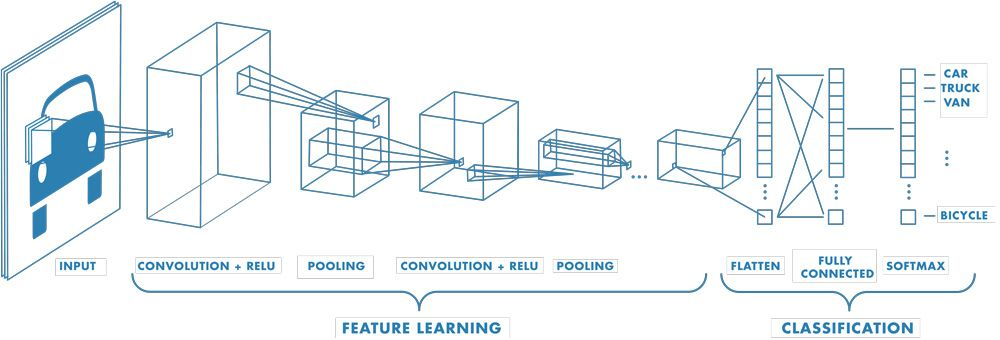
\includegraphics[scale=.45]{./Figures/cnn-image.jpeg}
	\caption{Ejemplo de arquitectura de red neuronal convolucional \cite{WEBSITE:2}.}
	\label{fig:cnn}
\end{figure}


\section{Detección de objetos}

La detección de objetos es una técnica utilizada en visión por computadora para localizar e identificar uno o varios objetos en una imagen o vídeo. A diferencia de otras técnicas de \textit{machine learning}, como es el caso de la clasificación o reconocimiento de imágenes, la detección busca localizar el lugar exacto donde se encuentra el objeto de interés y lo delimita con un rectángulo también llamado caja delimitadora o \textit{bounding box} por su término en inglés. Por otro lado, una vez delimitado el objeto se clasifica entre las categorías disponibles \cite{WEBSITE:5}.

La detección de objetos se puede implementar utilizando métodos de \textit{machine learning} clásicos o de \textit{deep learning}, dependiendo del problema a resolver\cite{WEBSITE:6}. El uso de \textit{deep learning} es más eficaz cuando se requiere tratar imágenes con muchas etiquetas, es decir, muchos objetos a detectar y las imágenes tienen otras variaciones como cambio de brillo, rotaciones, cambio de escala, etc. Por otro lado, el uso de \textit{machine learning} clásico es favorable cuando no se tienen altas capacidades de procesamiento y el número de etiquetas distintas a identificar es menor.

Algunos ejemplos de detección de objetos con \textit{machine learning} clásico son \textit{SIFT}, \textit{Temple Matching}, etc. En la figura \ref{fig:tempMatch}, se puede observar el uso de \textit{Temple Matching} para detectar el logo de Coca-Cola en una imagen.

\begin{figure}[ht]
	\centering
	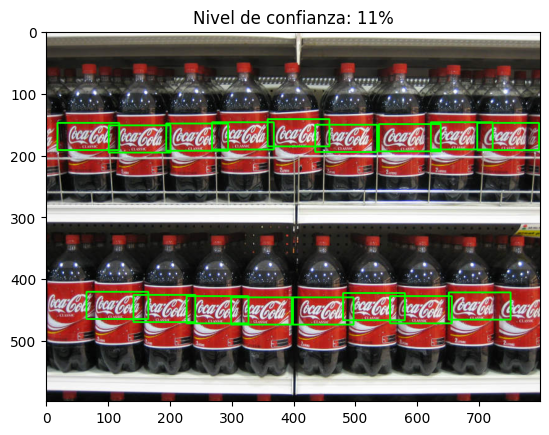
\includegraphics[scale=.45]{./Figures/template_match.png}
	\caption{Ejemplo de \textit{template matching} para identificar el logo de Coca-Cola.}
	\label{fig:tempMatch}
\end{figure}

Por otro lado, se tienen métodos de \textit{deep learning} para detección de objetos más avanzados que involucran detectores de dos etapas y de una etapa como son \textit{R-CNN}, \textit{Faster R-CNN}, \textit{SSD}, \textit{YOLO}, entre otros.

\subsection{Detectores de dos etapas}

Los detectores de dos etapas, como \textit{R-CNN} y sus variantes, primero extraen las características de la imagen y se propone la región de interés (ROI). El ROI, consiste en un \textit{bounding box} donde se presume que se encuentra el objeto a buscar. Luego, en la segunda etapa, se analizan las características encontradas en conjunto con el ROI, para seleccionar los \textit{bounding boxes} finales y calcular las probabilidades de que el objeto en las regiones pertenezca a una clase especifica \cite{ARTICLE:8}. 

Las redes neuronales de dos etapas son muy precisas al momento de detectar un objeto, sin embargo, son redes que son consideradas lentas durante la inferencia. Esta desventaja llevó a mejorar los modelos iniciales como \textit{R-CNN} a sus variantes \textit{Fast R-CNN} y \textit{Faster R-CNN}.

En la figura \ref{fig:rcnn}, se puede observar la arquitectura de una red neuronal de dos etapas \textit{R-CNN}.

\begin{figure}[ht]
	\centering
	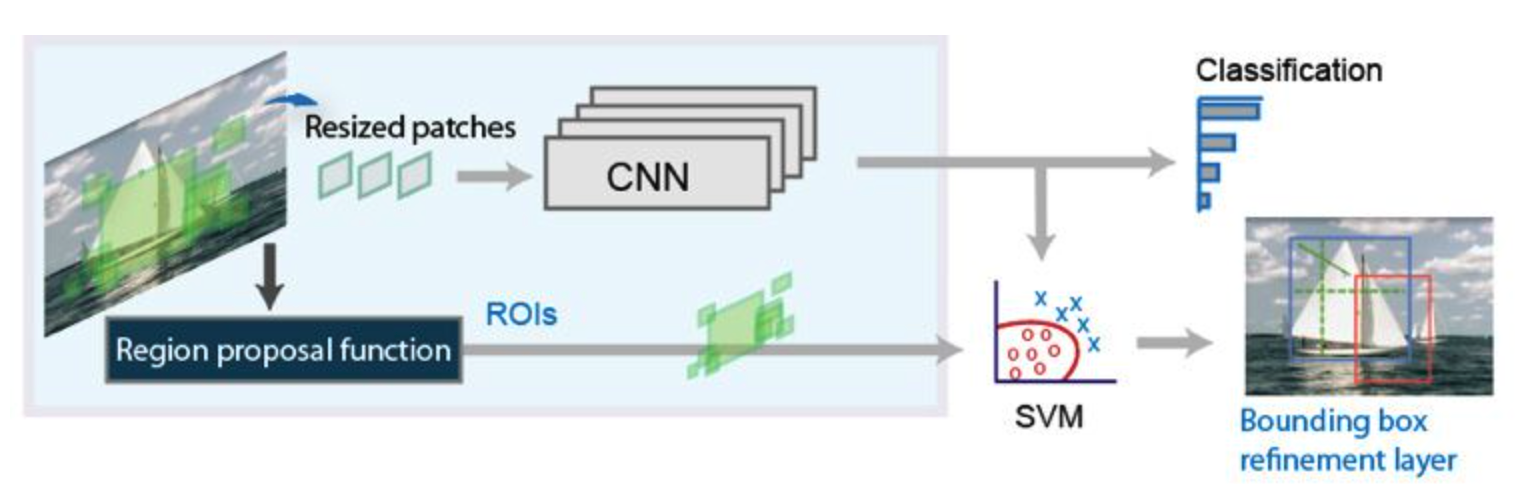
\includegraphics[scale=.25]{./Figures/R-CNN.png}
	\caption{Ejemplo de arquitectura de red neuronal de dos etapas \textit{R-CNN} \cite{WEBSITE:6}.}
	\label{fig:rcnn}
\end{figure}

\subsubsection{Detección de objetos con \textit{Fast R-CNN}}

Las mejoras adicionadas en \textit{Fast R-CNN} en comparación con \textit{R-CNN} incluyen una nueva capa llamada \textit{ROI Pooling}, que se encarga de extraer vectores de características de igual longitud de todas las regiones de interés propuestas. Por otro lado, \textit{R-CNN} contiene tres etapas como son la generación de región propuesta, la extracción de características y la clasificación usando \textit{SVM}, sin embargo, \textit{Fast R-CNN} crea una red neuronal que tiene una única etapa, reduciendo así el número de etapas de su predecesor. Además, este modelo comparte cálculos computacionales a través de todas las ROIs propuestas en vez de hacerlo una a una de manera independiente. Por último, \textit{Fast R-CNN} no guarda en cache las características, lo que reduce el uso de disco de memoria \cite{ARTICLE:10}.

\subsubsection{Detección de objetos con \textit{Faster R-CNN}}

El modelo \textit{Faster R-CNN} fue diseñado para superar muchos de los errores encontrados en sus predecesores como \textit{Fast R-CNN} y \textit{R-CNN}, en general como su nombre en inglés sugiere, sus mejoras van relacionadas a la rapidez en comparación a las otras variantes.

\textit{Faster R-CNN} mejora con respecto a \textit{Fast R-CNN} incorporando la red de región propuesta o por sus siglas en ingles RPN, que es una red completamente convolucional que produce propuestas con diferentes escalas y relaciones de aspecto. La RPN aplica la terminología de redes neuronales con atención para indicar al modelo a donde mirar.

En \textit{Faster R-CNN} se introduce el concepto de \textit{anchor boxes}, lo que permite detectar objetos en distintas escalas y relaciones de aspecto. Por último, se comparten cálculos computacionales a través de la RPN y \textit{Fast R-CNN}, lo que reduce el tiempo computacional \cite{ARTICLE:9}. En la figura \ref{fig:Faster-rcnn}, se muestra un ejemplo de la arquitectura de \textit{Faster R-CNN}.

\begin{figure}[ht]
	\centering
	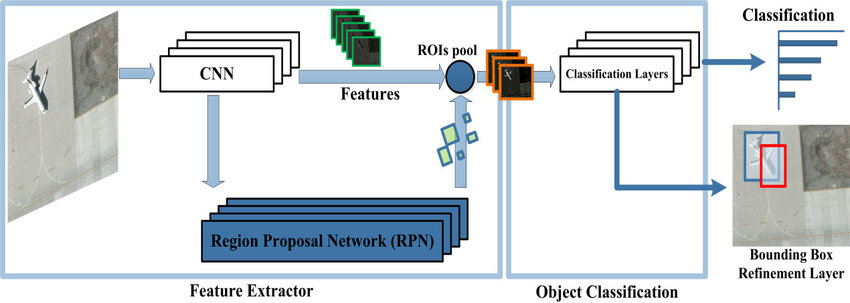
\includegraphics[scale=1.3]{./Figures/Faster-rcnn.png}
	\caption{Ejemplo de arquitectura de red neuronal de dos etapas \textit{Faster R-CNN} \cite{ARTICLE:11}.}
	\label{fig:Faster-rcnn}
\end{figure}

\subsection{Detectores de una etapa}

Los detectores de una etapa son modelos que omiten la etapa de RPN y ejecutan la detección directamente en un muestreo denso de ubicaciones. Estos modelos hacen uso de \textit{grid-box} y \textit{anchor box} para localizar la región de detección y delimitar al objeto de interés. En general, se consideran más rápidos que los detectores de dos etapas, sin embargo, son menos precisos \cite{ARTICLE:12}.

Algunos ejemplos de detectores de una etapa son las arquitecturas \textit{YOLO} \cite{ARTICLE:13}, \textit{SSD} \cite{ARTICLE:14}, \textit{RetinaNet} \cite{ARTICLE:15} y \textit{SqueezeDet} \cite{ARTICLE:16}. 

\subsubsection{Detección de objetos con \textit{YOLO}}

\textit{You Only Look Once} (\textit{YOLO}) es considerado el estado del arte para la detección en tiempo real y fue introducido en el año 2015. En el paper \cite{ARTICLE:13}, los autores trataron la detección de objetos como un problema de regresión simple en vez de hacerlo como un problema de clasificación, donde, se separa espacialmente los \textit{bounding boxes} y se les asocia una probabilidad a cada detección usando una red neuronal convolucional.

El algoritmo se basa en el uso de bloques residuales, \textit{bounding boxes} por regresión, \textit{Intersection Over Unions} (\textit{IoU}) y \textit{Non-Maximum Suppression}.

El primer paso es el uso de bloques residuales que consiste en dividir la imagen original en celdas cuadriculadas de NxN de igual dimensión. Cada celda en la cuadrícula es responsable de localizar y predecir la clase de objeto que cubre con su respectivo valor de confianza. Luego, se determinan los \textit{bounding boxes} con los atributos que \textit{YOLO} obtiene usando un módulo de regresión lineal. La respuesta que se recibe de este módulo es una representación vectorial de las coordenadas para cada \textit{bounding box}.

Por otro lado, un mismo objeto puede tener múltiples detecciones durante la predicción y no todas serán relevantes. Por este motivo, se usa \textit{Intersection Over Unions} que ayuda a descartar aquellas predicciones no relevantes, dándoles un valor entre 0 y 1. En este proceso, se establece un umbral para el \textit{Intersection Over Unions}, que posteriormente, se compara con el calculo generado por \textit{YOLO} para cada cuadrícula y si el resultado es menor al umbral establecido, se descarta dicha predicción. Por último, se aplica \textit{Non-Maximum Suppression} para preservar solo aquellas predicciones que tengan un valor de confianza alto \cite{WEBSITE:7}.

\textit{YOLO} cuenta con varias versiones desde su lanzamiento donde se ha mejorado su velocidad, precisión y el uso de recursos. Estas versiones, van desde la uno a la nueve, siendo la ocho la usada en la presente memoria.

\section{Clasificación de imágenes}

La clasificación de imágenes es una tarea fundamental en el ámbito de la visión por computadora, que consiste en asignar etiquetas o clases a las imágenes. Este proceso implica trabajar a nivel de píxeles, donde se extraen características de la imagen en formato vectorial, que luego son utilizadas por modelos de \textit{machine learning} para realizar predicciones. 

La clasificación puede llevarse a cabo mediante métodos de \textit{machine learning} clásicos o utilizando \textit{deep learning}. El uso de \textit{deep learning} para esta tarea ha demostrado un rendimiento sobresaliente, incluso ante imágenes con cambios de iluminación, rotación, deformación, oclusión, entre otros desafíos.

La clasificación de imágenes mediante \textit{deep learning} emplea redes neuronales convolucionales, un proceso que inicia con una imagen que pasa por una capa de entrada, donde se realiza un preprocesamiento antes de ser enviada a una capa convolucional. En la capa convolucional, se aplican filtros a la imagen para extraer características y generar un mapa de características que indica la presencia o ausencia de ciertos atributos. Posteriormente, la imagen se somete a una reducción de dimensionalidad en una capa de agrupación, de esta forma se preserva la información importante extraída, antes de pasar por una capa de activación no lineal, generalmente una capa ReLU. Finalmente, el resultado se alimenta a una capa totalmente conectada para obtener las probabilidades de que la imagen pertenezca a una de las clases predefinidas. En la figura \ref{fig:clasificación}, se puede observar un ejemplo del uso de deep learning en clasificación de imágenes.

\begin{figure}[ht]
	\centering
	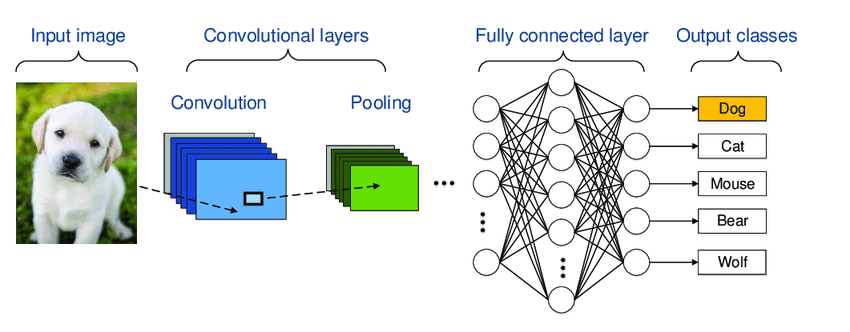
\includegraphics[scale=.32]{./Figures/image_classification.png}
	\caption{Clasificación de imagenes con \textit{deep learning} \cite{WEBSITE:8}.}
	\label{fig:clasificación}
\end{figure}



%\subsection{Uso de mayúscula inicial para los título de secciones}
%
%Si en el texto se hace alusión a diferentes partes del trabajo referirse a ellas como capítulo, sección o subsección según corresponda. Por ejemplo: ``En el capítulo \ref{Chapter1} se explica tal cosa'', o ``En la sección \ref{sec:ejemplo} se presenta lo que sea'', o ``En la subsección \ref{subsec:ejemplo} se discute otra cosa''.
%
%Cuando se quiere poner una lista tabulada, se hace así:
%
%\begin{itemize}
%	\item Este es el primer elemento de la lista.
%	\item Este es el segundo elemento de la lista.
%\end{itemize}
%
%Notar el uso de las mayúsculas y el punto al final de cada elemento.
%
%Si se desea poner una lista numerada el formato es este:
%
%\begin{enumerate}
%	\item Este es el primer elemento de la lista.
%	\item Este es el segundo elemento de la lista.
%\end{enumerate}
%
%Notar el uso de las mayúsculas y el punto al final de cada elemento.
%
%\subsection{Este es el título de una subsección}
%\label{subsec:ejemplo}
%
%Se recomienda no utilizar \textbf{texto en negritas} en ningún párrafo, ni tampoco texto \underline{subrayado}. En cambio sí se debe utilizar \textit{texto en itálicas} para palabras en un idioma extranjero, al menos la primera vez que aparecen en el texto. En el caso de palabras que estamos inventando se deben utilizar ``comillas'', así como también para citas textuales. Por ejemplo, un \textit{digital filter} es una especie de ``selector'' que permite separar ciertos componentes armónicos en particular.
%
%La escritura debe ser impersonal. Por ejemplo, no utilizar ``el diseño del firmware lo hice de acuerdo con tal principio'', sino ``el firmware fue diseñado utilizando tal principio''. 
%
%El trabajo es algo que al momento de escribir la memoria se supone que ya está concluido, entonces todo lo que se refiera a hacer el trabajo se narra en tiempo pasado, porque es algo que ya ocurrió. Por ejemplo, "se diseñó el firmware empleando la técnica de test driven development".
%
%En cambio, la memoria es algo que está vivo cada vez que el lector la lee. Por eso transcurre siempre en tiempo presente, como por ejemplo:
%
%``En el presente capítulo se da una visión global sobre las distintas pruebas realizadas y los resultados obtenidos. Se explica el modo en que fueron llevados a cabo los test unitarios y las pruebas del sistema''.
%
%Se recomienda no utilizar una sección de glosario sino colocar la descripción de las abreviaturas como parte del mismo cuerpo del texto. Por ejemplo, RTOS (\textit{Real Time Operating System}, Sistema Operativo de Tiempo Real) o en caso de considerarlo apropiado mediante notas a pie de página.
%
%Si se desea indicar alguna página web utilizar el siguiente formato de referencias bibliográficas, dónde las referencias se detallan en la sección de bibliografía de la memoria, utilizado el formato establecido por IEEE en \citep{IEEE:citation}. Por ejemplo, ``el presente trabajo se basa en la plataforma EDU-CIAA-NXP \citep{CIAA}, la cual...''.
%
%\subsection{Figuras} 
%
%Al insertar figuras en la memoria se deben considerar determinadas pautas. Para empezar, usar siempre tipografía claramente legible. Luego, tener claro que \textbf{es incorrecto} escribir por ejemplo esto: ``El diseño elegido es un cuadrado, como se ve en la siguiente figura:''
%
%\begin{figure}[h]
%\centering
%\includegraphics[scale=.45]{./Figures/cuadradoAzul.png}
%\end{figure}
%
%La forma correcta de utilizar una figura es con referencias cruzadas, por ejemplo: ``Se eligió utilizar un cuadrado azul para el logo, como puede observarse en la figura \ref{fig:cuadradoAzul}''.
%
%\begin{figure}[ht]
%	\centering
%	\includegraphics[scale=.45]{./Figures/cuadradoAzul.png}
%	\caption{Ilustración del cuadrado azul que se eligió para el diseño del logo.}
%	\label{fig:cuadradoAzul}
%\end{figure}
%
%El texto de las figuras debe estar siempre en español, excepto que se decida reproducir una figura original tomada de alguna referencia. En ese caso la referencia de la cual se tomó la figura debe ser indicada en el epígrafe de la figura e incluida como una nota al pie, como se ilustra en la figura \ref{fig:palabraIngles}.
%
%\begin{figure}[htpb]
%	\centering
%	\includegraphics[scale=.3]{./Figures/word.jpeg}
%	\caption{Imagen tomada de la página oficial del procesador\protect\footnotemark.}
%	\label{fig:palabraIngles}
%\end{figure}
%
%\footnotetext{Imagen tomada de \url{https://goo.gl/images/i7C70w}}
%
%La figura y el epígrafe deben conformar una unidad cuyo significado principal pueda ser comprendido por el lector sin necesidad de leer el cuerpo central de la memoria. Para eso es necesario que el epígrafe sea todo lo detallado que corresponda y si en la figura se utilizan abreviaturas entonces aclarar su significado en el epígrafe o en la misma figura.
%
%
%
%\begin{figure}[ht]
%	\centering
%	\includegraphics[scale=.37]{./Figures/questionMark.png}
%	\caption{¿Por qué de pronto aparece esta figura?}
%	\label{fig:questionMark}
%\end{figure}
%
%Nunca colocar una figura en el documento antes de hacer la primera referencia a ella, como se ilustra con la figura \ref{fig:questionMark}, porque sino el lector no comprenderá por qué de pronto aparece la figura en el documento, lo que distraerá su atención.
%
%Otra posibilidad es utilizar el entorno \textit{subfigure} para incluir más de una figura, como se puede ver en la figura \ref{fig:three graphs}. Notar que se pueden referenciar también las figuras internas individualmente de esta manera: \ref{fig:1de3}, \ref{fig:2de3} y \ref{fig:3de3}.
% 
%\begin{figure}[!htpb]
%     \centering
%     \begin{subfigure}[b]{0.3\textwidth}
%         \centering
%         \includegraphics[width=.65\textwidth]{./Figures/questionMark}
%         \caption{Un caption.}
%         \label{fig:1de3}
%     \end{subfigure}
%     \hfill
%     \begin{subfigure}[b]{0.3\textwidth}
%         \centering
%         \includegraphics[width=.65\textwidth]{./Figures/questionMark}
%         \caption{Otro.}
%         \label{fig:2de3}
%     \end{subfigure}
%     \hfill
%     \begin{subfigure}[b]{0.3\textwidth}
%         \centering
%         \includegraphics[width=.65\textwidth]{./Figures/questionMark}
%         \caption{Y otro más.}
%         \label{fig:3de3}
%     \end{subfigure}
%        \caption{Tres gráficos simples}
%        \label{fig:three graphs}
%\end{figure}
%
%El código para generar las imágenes se encuentra disponible para su reutilización en el archivo \file{Chapter2.tex}.
%
%\subsection{Tablas}
%
%Para las tablas utilizar el mismo formato que para las figuras, sólo que el epígrafe se debe colocar arriba de la tabla, como se ilustra en la tabla \ref{tab:peces}. Observar que sólo algunas filas van con líneas visibles y notar el uso de las negritas para los encabezados.  La referencia se logra utilizando el comando \verb|\ref{<label>}| donde label debe estar definida dentro del entorno de la tabla.
%
%\begin{verbatim}
%\begin{table}[h]
%	\centering
%	\caption[caption corto]{caption largo más descriptivo}
%	\begin{tabular}{l c c}    
%		\toprule
%		\textbf{Especie}     & \textbf{Tamaño} & \textbf{Valor}\\
%		\midrule
%		Amphiprion Ocellaris & 10 cm           & \$ 6.000 \\		
%		Hepatus Blue Tang    & 15 cm           & \$ 7.000 \\
%		Zebrasoma Xanthurus  & 12 cm           & \$ 6.800 \\
%		\bottomrule
%		\hline
%	\end{tabular}
%	\label{tab:peces}
%\end{table}
%\end{verbatim}
%
%
%\begin{table}[h]
%	\centering
%	\caption[caption corto]{caption largo más descriptivo}
%	\begin{tabular}{l c c}    
%		\toprule
%		\textbf{Especie} 	 & \textbf{Tamaño} 		& \textbf{Valor}  \\
%		\midrule
%		Amphiprion Ocellaris & 10 cm 				& \$ 6.000 \\		
%		Hepatus Blue Tang	 & 15 cm				& \$ 7.000 \\
%		Zebrasoma Xanthurus	 & 12 cm				& \$ 6.800 \\
%		\bottomrule
%		\hline
%	\end{tabular}
%	\label{tab:peces}
%\end{table}
%
%En cada capítulo se debe reiniciar el número de conteo de las figuras y las tablas, por ejemplo, figura 2.1 o tabla 2.1, pero no se debe reiniciar el conteo en cada sección. Por suerte la plantilla se encarga de esto por nosotros.
%
%\subsection{Ecuaciones}
%\label{sec:Ecuaciones}
%
%Al insertar ecuaciones en la memoria dentro de un entorno \textit{equation}, éstas se numeran en forma automática  y se pueden referir al igual que como se hace con las figuras y tablas, por ejemplo ver la ecuación \ref{eq:metric}.
%
%\begin{equation}
%	\label{eq:metric}
%	ds^2 = c^2 dt^2 \left( \frac{d\sigma^2}{1-k\sigma^2} + \sigma^2\left[ d\theta^2 + \sin^2\theta d\phi^2 \right] \right)
%\end{equation}
%                                                        
%Es importante tener presente que si bien las ecuaciones pueden ser referidas por su número, también es correcto utilizar los dos puntos, como por ejemplo ``la expresión matemática que describe este comportamiento es la siguiente:''
%
%\begin{equation}
%	\label{eq:schrodinger}
%	\frac{\hbar^2}{2m}\nabla^2\Psi + V(\mathbf{r})\Psi = -i\hbar \frac{\partial\Psi}{\partial t}
%\end{equation}
%
%Para generar la ecuación \ref{eq:metric} se utilizó el siguiente código:
%
%\begin{verbatim}
%\begin{equation}
%	\label{eq:metric}
%	ds^2 = c^2 dt^2 \left( \frac{d\sigma^2}{1-k\sigma^2} + 
%	\sigma^2\left[ d\theta^2 + 
%	\sin^2\theta d\phi^2 \right] \right)
%\end{equation}
%\end{verbatim}
%
%Y para la ecuación \ref{eq:schrodinger}:
%
%\begin{verbatim}
%\begin{equation}
%	\label{eq:schrodinger}
%	\frac{\hbar^2}{2m}\nabla^2\Psi + V(\mathbf{r})\Psi = 
%	-i\hbar \frac{\partial\Psi}{\partial t}
%\end{equation}
%
%\end{verbatim}